


\chapter{Duality}\label{chap:duality}

This section will now establish the connection that exists between multi-paths and multi-surfaces that will henceforth be referred to as ``duality".


\section{Point-volume duality}

To quantify a multi-point \(\rho\), at each position \(\mathbf{q}\) only one value \(\rho(\mathbf{q})\) is required. 

To quantify a multi-volume \(U\), at each position \(\mathbf{q}\) only one value \(U(\mathbf{q})\) is also required. 

The fact that multi-points and multi-volumes both only require 1 value suggests that points and volumes can be ``interchanged". When a multi-point and a multi-volume are interchangeable, they will be referred to as being ``dual" to each other.

\begin{tabular}{cc}
\parbox{0.5\textwidth}{
Given a point \(P\) with an {\bf infinitesimal} weight of \(w\), then the volume that is ``dual" to \(P\) is an infinitesimal volume \(\Omega\) that both contains \(P\) and has a volume of \(w\). 

Given an {\bf infinitesimal} volume \(\Omega\) with a volume of \(\Delta V\), then the point that is ``dual" to \(\Omega\) is a point \(P\) that is contained by \(\Omega\) and has a weight of \(\Delta V\).

Consider a multi-volume \(U\). Multi-volume \(U\) consists of a single volume with a weight of \(1\). The multi-point \(\rho\) that is ``dual" to \(\Omega\) is a uniform ``cloud" of points each with an infinitesimal weight. The average total weight per unit volume is \(1\). In the image on the right, a large volume is shattered into infinitesimal volumes, each shard of which is dual to point with a weight equal to the volume of said shard. 
} & \parbox{0.5\textwidth}{
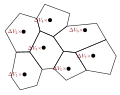
\includegraphics[width = 0.5\textwidth]{Duality/point_volume_duality}
}
\end{tabular}

While there is no unique way of exactly placing the dual points or sketching the dual volumes, once ``smoothing" has been applied none of this matters.

Given a multi-volume \(U\), the multi-point \(\rho\) that is ``dual" to \(U\) will be denoted via the notation:
\[\rho = \iota(U)\]
or conversely, 
\[U = \iota^{-1}(\rho)\]

The following is important to note:
\begin{itemize}
\item The dual of the union is the union of the duals:
\[\iota(U_1 + U_2) = \iota(U_1) + \iota(U_2)
\quad\quad\text{and}\quad\quad
\iota^{-1}(\rho_1 + \rho_2) = \iota^{-1}(\rho_1) + \iota^{-1}(\rho_2)\]
If \(c\) is an arbitrary real valued coefficient, then:
\[\iota(c \cdot U) = c \cdot \iota(U)
\quad\quad\text{and}\quad\quad
\iota^{-1}(c \cdot \rho) = c \cdot \iota^{-1}(\rho)\]
\end{itemize}




\section{Path-surface duality}

To quantify a multi-path \(\mathbf{J}\), at each position \(\mathbf{q}\) three values \(\begin{bmatrix} J_1(\mathbf{q}) \\ J_2(\mathbf{q}) \\ J_3(\mathbf{q}) \end{bmatrix}\) are required. 

To quantify a multi-surface \(\mathbf{F}\), at each position \(\mathbf{q}\) three values \(\begin{bmatrix} F_1(\mathbf{q}) \\ F_2(\mathbf{q}) \\ F_3(\mathbf{q}) \end{bmatrix}\) are also required. 

The fact that multi-paths and multi-surface both require 3 values suggests that paths and surfaces can be ``interchanged". When a multi-path and multi-surface are interchangeable, they will be referred to as being ``dual" to each other.

Given an infinitesimal segment of path \(C\) with an infinitesimal weight, the surface \(\sigma\) that is ``dual" to \(C\) is: 
\begin{itemize}
\item Infinitesimal in both size and weight.
\item Perpendicular to \(C\). 
\item The direction of \(C\) passes through \(\sigma\) in the preferred direction. This gives the intersections of dual paths and surfaces positive weight. 
\end{itemize}

To visualize a smoothed multi-path and its smoothed dual surface, sheath the infinitesimal path fibers in a cylinder. The path fibers are parallel to the sides of the cylinder, and are perpendicular to the end caps. The dual surfaces are perpendicular to the sides of the cylinder and are parallel to the end caps. The total path weight passing through the cylinder is proportional to the cross-sectional area of the cylinder, while the total surface weight slicing through the cylinder is proportional to its length.

In the image below, the leftmost cylinders contain a path with a total weight of \(w_{\parallel}\), and a surface with a total weight of \(w_{\perp}\). These paths and surfaces are dual to each other. In the top row of images, when the cylinder decreases in length, the contained surface weight decreases proportionally, while the contained path weight remains constant. In the bottom row of images, when the cylinder decreases in cross-sectional area, the contained path weight decreases proportionally, while the contained surface weight remains constant. 

\begin{center}
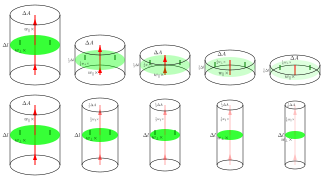
\includegraphics[width = 0.9\textwidth]{Duality/path_surface_duality_2}
\end{center}

To determine the multi-path \(\mathbf{J}\) that is dual to a multi-surface \(\mathbf{F}\), break the multi-surface \(\mathbf{F}\) into infinitesimal sections with equal weight and area, replace each section of surface with its dual path, and lastly stitch the path segments together leaving as little endpoints as possible. While there is no unique way of performing this process, once ``smoothing" has been applied none of this matters.  

\begin{center}
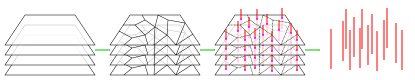
\includegraphics[width = 0.9\textwidth]{Duality/path_surface_duality_3}
\end{center}

Given a multi-surface \(\mathbf{F}\), the multi-path \(\mathbf{J}\) that is ``dual" to \(\mathbf{F}\) will be denoted via the notation:
\[\mathbf{J} = \epsilon(\mathbf{F})\]
or conversely, 
\[\mathbf{F} = \epsilon^{-1}(\mathbf{J})\]

The following is important to note:
\begin{itemize}
\item The dual of the union is the union of the duals:
\[\epsilon(\mathbf{F}_1 + \mathbf{F}_2) = \epsilon(\mathbf{F}_1) + \epsilon(\mathbf{F}_2)
\quad\quad\text{and}\quad\quad
\epsilon^{-1}(\mathbf{J}_1 + \mathbf{J}_2) = \epsilon^{-1}(\mathbf{J}_1) + \epsilon^{-1}(\mathbf{J}_2)\]
If \(c\) is an arbitrary real valued coefficient, then:
\[\epsilon(c \cdot \mathbf{F}) = c \cdot \epsilon(\mathbf{F})
\quad\quad\text{and}\quad\quad
\epsilon^{-1}(c \cdot \mathbf{J}) = c \cdot \epsilon^{-1}(\mathbf{J})\]
\end{itemize}



\section{Duality and intersections}

\begin{thm}
Given multi-point \(\rho\) and multi-volume \(V\), 

\[\iota^{-1}(\rho \cdot V) = \iota^{-1}(\rho) \cdot V\]

Given multi-point \(\mathbf{J}\) and multi-volume \(V\), 

\[\epsilon^{-1}(\mathbf{J} \cdot V) = \epsilon^{-1}(\mathbf{J}) \cdot V\]

Given multi-surface \(\mathbf{F}\) and multi-volume \(V\), 

\[\epsilon(\mathbf{F} \cdot V) = \epsilon(\mathbf{F}) \cdot V\]

Given multi-volume \(U\) and multi-volume \(V\), 

\[\iota(U \cdot V) = \iota(U) \cdot V\]
\end{thm}


\begin{tabular}{cc}
\parbox{0.5\textwidth}{
\begin{thm}
Given multi-volumes \(U\) and \(V\),

\[\iota(U) \cdot V = U \cdot \iota(V)\]
\end{thm}
} & \parbox{0.5\textwidth}{
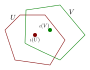
\includegraphics[width = 0.5\textwidth]{Duality/point_volume_duality_intersection}
}
\end{tabular}


\begin{tabular}{cc}
\parbox{0.5\textwidth}{
\begin{thm}
Given multi-surfaces \(\mathbf{F}\) and \(\mathbf{G}\), 

\[\epsilon(\mathbf{F}) \bullet \mathbf{G} = \mathbf{F} \bullet \epsilon(\mathbf{G})\]
\end{thm}
} & \parbox{0.5\textwidth}{
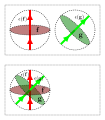
\includegraphics[width = 0.5\textwidth]{Duality/path_surface_duality_intersection}
}
\end{tabular}



%Given multi-paths \(\mathbf{J}\) and \(\mathbf{K}\), and multi-surface \(\mathbf{F}\), then:
%
%\[\mathbf{F} \times \epsilon^{-1}(\epsilon^{-1}(\mathbf{J}) \times \epsilon^{-1}(\mathbf{K})) = \iota^{-1}(\mathbf{F} \bullet \mathbf{K})\mathbf{J} - \iota^{-1}(\mathbf{F} \bullet \mathbf{J})\mathbf{K}\]
%
%\begin{tabular}{cc}
%\parbox{0.5\textwidth}{
%\includegraphics[width = 0.5\textwidth]{Duality/triple_vector_product_tetrahedron_F_dot_J=0}
%} & \parbox{0.5\textwidth}{
%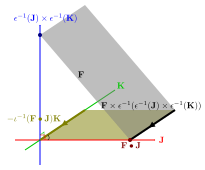
\includegraphics[width = 0.5\textwidth]{Duality/triple_vector_product_tetrahedron_F_dot_K=0}
%} 
%\end{tabular}
%
%\begin{center}
%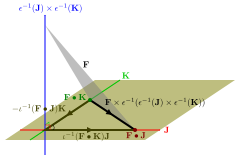
\includegraphics[width = 0.75\textwidth]{Duality/triple_vector_product_tetrahedron}
%\end{center}





\section{Energy}

\subsection{Path energy}

Given a multi-path \(\mathbf{D}\), the ``energy" of \(\mathbf{D}\) is \(1/2\) the total number of intersections that the path has with its own dual:

\[E = \frac{1}{2}\int (\mathbf{D} \bullet \epsilon^{-1}(\mathbf{D}))\]

The multiplier of \(\frac{1}{2}\) exists to remain consistent with physics.

The energy is always strictly positive except for the \(0\) multi-path where the energy is \(0\).


\subsection{Surface energy}

Given a multi-surface \(\mathbf{E}\), the ``energy" of \(\mathbf{E}\) is \(1/2\) the total number of intersections that the surface has with its own dual:

\[E = \frac{1}{2}\int (\epsilon(\mathbf{E}) \bullet \mathbf{E})\]

Again, the multiplier of \(\frac{1}{2}\) exists to remain consistent with physics.

The energy is always strictly positive except for the \(0\) multi-surface where the energy is \(0\).


\subsection{Loop-bubble duality}


If a multi-bubble is dual to a multi-loop, then both are \(0\). This can be proven from  the fact that the energy of a nonzero path or surface is always positive. 

\begin{thm}\label{thm:loop_bubble_duality}
Assume that \(\mathbf{E}\) is a multi-bubble: \(\nabla \times \mathbf{E} = 0\). Also assume that the dual multi-path \(\mathbf{D} = \epsilon(\mathbf{E})\) is also a multi-loop: \(\nabla \bullet \mathbf{D} = 0\). It must then be the case that \(\mathbf{E} = 0\) and \(\mathbf{D} = 0\).
\end{thm}
\textbf{Proof:}

Since \(\mathbf{E}\) is a multi-bubble, there must exist some multi-volume \(U\) whose inwards oriented surface is \(\mathbf{E}\). 

The energy of both \(\mathbf{D}\) and \(\mathbf{E}\) is:

\begin{align*}
E = & \frac{1}{2}\int (\mathbf{D} \bullet \mathbf{E}) 
= \frac{1}{2} \int (\mathbf{D} \bullet (\nabla U)) 
\end{align*} 

As discussed in section \ref{sec:endpoints_of_path_volume_intersect}, the number of times \(\mathbf{D}\) enters \(U\) is the total number of finishing points \(\mathbf{D}\) leaves in \(U\) so: 
\[\int (\mathbf{D} \bullet (\nabla U)) = -\int ((\nabla \bullet \mathbf{D}) U)\] 
therefore continuing the derivation yields:

\begin{align*}
E = & \frac{1}{2} \int (\mathbf{D} \bullet (\nabla U)) 
= -\frac{1}{2} \int ((\nabla \bullet \mathbf{D}) U) 
= -\frac{1}{2} \int (0 \cdot U) 
= 0
\end{align*}

The energy is \(0\), and this only occurs if \(\mathbf{D} = 0\) and \(\mathbf{E} = 0\). {\bf Non-zero multi-bubbles can never be dual to a multi-loop and vice versa. \(\Box\)}


A consequence of this fact is that if two path-surface pairs have the same end-points and counterclockwise boundaries, then they are equivalent: 

\begin{cor}\label{cor:loop_bubble_duality}
Let \(\mathbf{D}_1\) and \(\mathbf{E}_1\) be a multi-path and a multi-surface pair that are dual to each other: \(\mathbf{D}_1 = \epsilon(\mathbf{E}_1)\)

Let \(\mathbf{D}_2\) and \(\mathbf{E}_2\) also be a multi-path and a multi-surface pair that are dual to each other: \(\mathbf{D}_2 = \epsilon(\mathbf{E}_2)\)

If \(\nabla \bullet \mathbf{D}_1 = \nabla \bullet \mathbf{D}_2\) and \(\nabla \times \mathbf{E}_1 = \nabla \times \mathbf{E}_2\), then \(\mathbf{D}_1 = \mathbf{D}_2\) and \(\mathbf{E}_1 = \mathbf{E}_2\).   
\end{cor}
\textbf{Proof:}

Let \(\mathbf{D}_{\text{loop}} = \mathbf{D}_1 - \mathbf{D}_2\). \(\mathbf{D}_{\text{loop}}\) is a multi-loop:
\[\nabla \bullet \mathbf{D}_{\text{loop}} = \nabla \bullet (\mathbf{D}_1 - \mathbf{D}_2) = \nabla \bullet \mathbf{D}_1 - \nabla \bullet \mathbf{D}_2 = 0\]

Let \(\mathbf{E}_{\text{bubble}} = \mathbf{E}_1 - \mathbf{E}_2\). \(\mathbf{E}_{\text{bubble}}\) is a multi-bubble: 
\[\nabla \times \mathbf{E}_{\text{bubble}} = \nabla \times (\mathbf{E}_1 - \mathbf{E}_2) = \nabla \times \mathbf{E}_1 - \nabla \times \mathbf{E}_2 = 0\]

\(\mathbf{D}_{\text{loop}}\) and \(\mathbf{E}_{\text{bubble}}\) are a dual pair:
\[\epsilon(\mathbf{E}_{\text{bubble}}) = \epsilon(\mathbf{E}_1 - \mathbf{E}_2) = \epsilon(\mathbf{E}_1) - \epsilon(\mathbf{E}_2) = \mathbf{D}_1 - \mathbf{D}_2 = \mathbf{D}_{\text{loop}}\]

From theorem \ref{thm:loop_bubble_duality}, \(\mathbf{D}_{\text{loop}} = 0\) and \(\mathbf{E}_{\text{bubble}} = 0\). Therefore \(\mathbf{D}_1 = \mathbf{D}_2\) and \(\mathbf{E}_1 = \mathbf{E}_2\). \(\Box\)



\subsection{Low energy solutions}

Given a balanced multi-point \(\rho\), it is known via theorem \ref{thm:dot-to-dot} from section \ref{sec:balanced_multi-points} that there must exist a multi-path \(\mathbf{D}\) such that \(\nabla \bullet \mathbf{D} = \rho\). However, the choice of \(\mathbf{D}\) is {\bf not unique}. A unique choice of \(\mathbf{D}\) is the choice that minimizes the energy \(\frac{1}{2}\int (\mathbf{D} \bullet \epsilon^{-1}(\mathbf{D}))\). It will now be demonstrated that the energy minimizing choice is both unique and is dual to a multi-bubble:

\begin{thm}
Given a balanced multi-point \(\rho\), the multi-path \(\mathbf{D}\) that satisfies \(\nabla \bullet \mathbf{D} = \rho\) and minimizes the energy \(\frac{1}{2}\int (\mathbf{D} \bullet \epsilon^{-1}(\mathbf{D}))\) is both {\bf unique} and is dual to a multi-bubble: \(\nabla \times \epsilon^{-1}(\mathbf{D}) = 0\). 
\end{thm}
\textbf{Proof:}




\section{Inductance}



\section{Electrostatics and magnetostatics}








